\documentclass{article}
\usepackage[a4paper, portrait, margin=2cm]{geometry}
\usepackage[utf8]{inputenc}
\usepackage{appendix}
\usepackage{url}
\usepackage{bchart}
\usepackage{minted}
\usepackage{graphicx}
\usepackage{pgfplots}
\usepackage{booktabs}
\usepackage{graphicx}
\usepackage[table,xcdraw]{xcolor}
\graphicspath{ {./images/} }
\title{\textbf{Predicting bitcoin prices from Twitter sentiment analysis}}
\author{Fran Jurinec, Thinh Lam, Emilia Marchese}
\date{October 2021}

\begin{document}

\maketitle

\section{Introduction}
The goal of this project is to research the ability to predict Bitcoin price movement using social media sentiment data and historical price data. The first stage of the project focuses on collecting social media content over a large time period with a goal of creating a time series representation of sentiment. Once this data is obtained, in the second stage of the project, we will evaluate the feasibility of predicting bitcoin price changes using this data via a number of different prediction models. 

The end goal of this project is to deploy a customer facing application which will use the optimal prediction model to present price predictions to end users.
The application will also provide users with additional information about sentiment and historical overviews of the data to allow them to make more informed trading decisions.


\section{Twitter sentiment analysis}
\subsection{Data Wrangling}

The data we got for this project are Twitters tweet data and Bitcoin price history data.  Originally, we wanted to get the twitter data from twitter API, but we run into some trouble. So, we ended up using Kaggles Bitcoin Tweets dataset, whose source is also gathered from Twitter API. This dataset contains all tweets that have the word \#bitcoin and \#btc from year 2016 to 2019.

During the data process we removed all unnecessary columns, like “user\_name”, “user\_verified”, “user\_followers”, etc. and chose 3 columns that are necessary for the sentiment analysis. Those are “timestamp”, “text” and “likes”. We also decided to drop all tweets that have under one like, because we thought that they were insignificant in our sentiment analysis. 

\subsection{VADER}

Sentiment analysis also known as opinion mining is the process of determining whether the analyzing text is in our case positive or negative. This is widely applied in business, politics, and public actions.

The sentiment analyzer we used in our project is Valence Aware Dictionary and Sentiment Reasoner (VADER). VADER is a parsimonious rule-based model that is commonly used for analyzing sentiment in social media [1].

We get sentiment from VADER with the polarity\_scores function and extracted compound from the results. The compound is the sentiment metric that is computed with VADERs lexicon ratings and rules, and which is normalized to values between -1 (negative) and 1 (positive). With compound we can see how positive or negative the text is. So, we analyzed every tweets text and got a compound score for every tweet. 

\subsection{Weekly Sentiment Calculations}

Next, we calculate the weekly sentiment. We grouped all tweets weekly and calculate every weeks sentiment mean with this formula  \[\frac{1}{n}\sum_{i=1}^{n}x_i\] where $x_i$ is i:th tweet. In this formula, we leave out all zero sentiment tweets. In other words the n in the formula is smaller and there are steeper ups and downs in the plot below. Also it removes random tweets with just a link from the calculation. 

\begin{figure}[h]
    \centering
    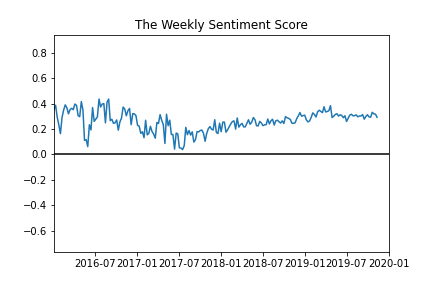
\includegraphics[scale=0.75]{WeeklySentiment.png}
    \caption{Weekly unweighted sentiment score time series}
    \label{fig:my_label}
\end{figure}


Later in the project we weren't satisfied with the results we generated with normal weekly sentiment, so we calculated weighted sentiment by likes and tested if we got better results. The formula to calculate the weighted sentiment by likes is 
\[\frac{1}{n}\sum_{i=1}^{n}w_ix_i\] where $x_i$ is sentiment and $w_i$ is likes in i:th tweet. In this we also removed zero sentiment tweets from the calculations.

\begin{figure}[h]
    \centering
    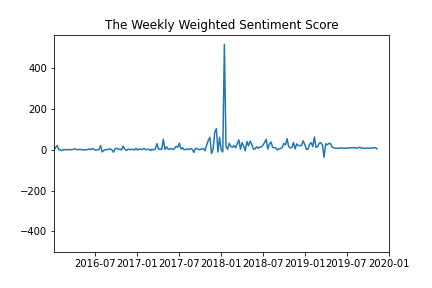
\includegraphics[scale=0.75]{WeeklyWeightedSentiment.png}
    \caption{Weekly Weighted sentiment score time series}
    \label{fig:my_label}
\end{figure}


Now the sentiment data is ready for models. 

\section{Models}

Several models were run. The aim was to use the past lags of both time series to forecast the bitcoin prices, rather than have the sentiment as the only predictor. This choice was made because, especially with stock prices, the past price values can be very indicative in predicting the future values. The models were trained first with unweighted sentiment and the prices, and later with the weighted sentiment and prices. The weighted sentiment resulted in better evaluation statistics, so it was decided to use that one as the sentiment time series. 
\subsection{Data pre-processing}
\subsubsection{Differencing and ADF}
A prerequisite of several time series analysis models is the necessity of having time series that are stationary. Time series are stationary if they do not have a trend or seasonal effects, which in empirical terms signifies that the series does not have a unit root. The presence of a unit root can be tested by using the Augmented-Dick-Fuller test, where the null hypothesis is that the time series does have a unit root and that it is therefore not stochastic.
The close price time series resulted to have a unit root, which was not unexpected. It was therefore decided to first-difference both time series to evaluate whether the resulting time series would be stationary. The ADF test was conducted on the first-differenced close and weighted sentiment time series. For both it was able to reject the null hypothesis at the 5\% significance level so the first-differenced series were deemed stationary and were used to train the model.
\subsubsection{Granger causality test}
The Granger causality test is a statistical hypothesis test for determining whether one time series is useful in forecasting another. The test was run on the two time series to evaluate whether the weighted sentiment would actually be useful in predicting the close bitcoin price. The p-value of the weighted sentiment causing the close price was less than 0.05, so the null hypothesis that the weighted sentiment had no effect on the close price was rejected and the weighted sentiment was deemed as an acceptable predictor for the close price.
\subsection{Running the models}
\subsection{Darts}
Initially the data was split so that the last 15 observations in the time series were kept as the test set, and all previous observations were allocated to the train set. All models were first trained with this train data and the forecast were made for the 15 observations. 
Most of the models were run using the library Darts (\url{https://github.com/unit8co/darts}). Five models were run in total, all of which were trained using both the time series of the price (so using the lag values of the price) and the time series of the weighted sentiment as predictors. Here below we describe some of the models used, putting more emphasis on the one that resulted in better predictions given our data: 
\begin{itemize}
    \item \textbf{VAR(VARIMA)}: Vector Autoregression (VAR) is a forecasting bidirectional algorithm that can be used when two or more time series influence each other. In our case, we decided to use the past 15 lags of the outcome variable price and the past 15 lags of the weighted sentiment as estimators (so the 15 weeks before the one we want to forecast). Of course the series were first differenced.
    The VAR equation for the price forecast is hence along the lines of: 
    \[P_{1,t} = \alpha + P_{t-1} + S_{t-1} + ... + P_{t-15} + S_{t-15} + \beta_{p,1} \Delta P_{t-1}+ \beta_{s,1} \Delta S_{t-1} + ... + \beta_{p,15} \Delta P_{t-15}+ \beta_{s, 15} \Delta S_{t-15}+ \epsilon_{p,t}\]
    Where $P$ is the bitcoin price, $t$ is the period and $S$ is the weighted sentiment and $\Delta$ stands for the first difference in lag $t$ (so $\Delta P_{t-1} = P_{t-1}-P_{t-2}$). 
    \item \textbf{NBEATS}: A neural basis expansion analysis for interpretable time series is a complex forecasting algorithm that is know for having outperformed well-established statistical approaches on the M3, and M4 competitions. A brief description of the model can be seen in Figure 3. More information can be found at \url{https://unit8co.github.io/darts/examples/08-NBEATS-examples.html}. 
    \begin{figure}[h]
        \centering
        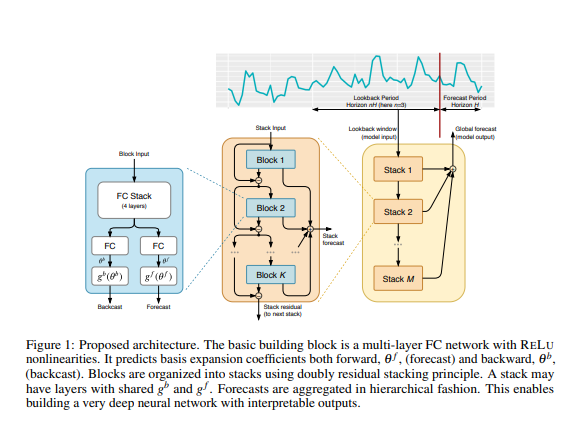
\includegraphics[width = 10cm]{NBEATS.png}
        \caption{NBEATS architecture}
        \label{fig:my_label}
    \end{figure}
    \item \textbf{TCNModel}: More information on the temporal convulsional networks can be found here \url{https://unit8co.github.io/darts/examples/06-TCN-examples.html}. 
    \item \textbf{BlockRNNModel}: More information on the BlockRNNModel can be found here: \url{https://unit8co.github.io/darts/examples/05-RNN-examples.html}.
    \item \textbf{TransformerModel}: More informaiton on the TransformerModel can be found here: \url{https://unit8co.github.io/darts/examples/07-Transformer-examples.html}.
\end{itemize}
Of these five models, the TransformerModel and the BlockRNNModel were immediately dismissed because they forecasted the same value for the 15 observations (see figures in Appendix, where you can observe an obvious straight line in the de-differentiated time series).The reasonable models (VAR, NBEATS and TCNModel) were evaluated using the MAPE (mean absulute prediction error) estimate on the forecast and the actual values kept in the test data (both de-differentiated). The model that achieved the best MAPE (NBEATS) was then used to as the model for the prediction that have been displayed in the application.
\begin{figure}[h]
    \centering
    \subfigure{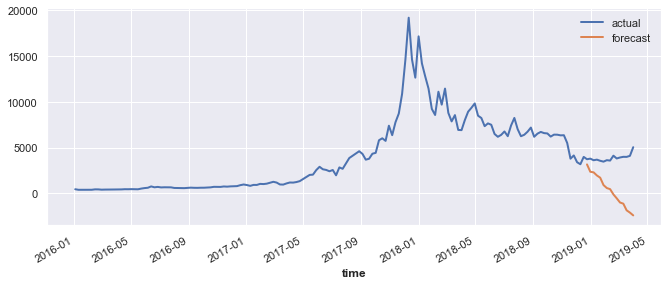
\includegraphics[width=0.3\textwidth]{predTCNM.png}} 
    \subfigure{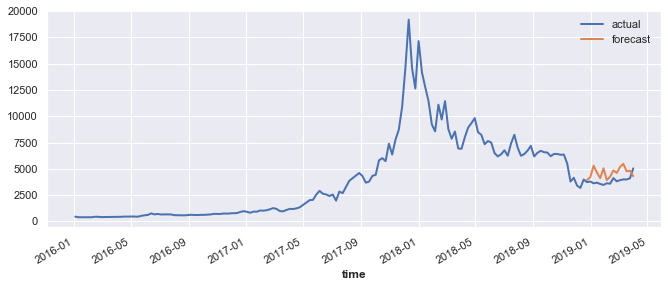
\includegraphics[width=0.3\textwidth]{var.png}} 
    \subfigure{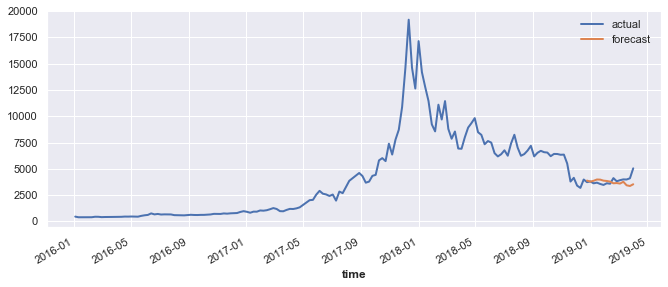
\includegraphics[width=0.3\textwidth]{BCNM.png}}
    \caption{(a) TCNModel (b) VARIMA (c) NBEATS}
    \label{fig:foobar}
\end{figure}

\begin{figure}[h]
\centering
    \begin{bchart}[max=100, unit = \%]
    \bcbar[text= a,color=yellow]{90.02}
    \bcbar[text= b,color=red!50]{22.48}
    \bcbar[text= c,color=green!60!blue]{9.77}
    \bcxlabel{MAPE for (a) TCNModel (b) VARIMA (c) NBEATS }
    \end{bchart}
\caption{MAPES for models}
\end{figure}

\section{Results}
The prediction in the application deployed to the user is only for the next week after the one selected, so the NBEATS model is trained on all the data points of close price and weighted sentiment previous to the week to forecast, and the output was the first-differences price observation for the next week which is used to show the change in price for the next week. The dates for which the user can select the forecast were chosen randomly from the time series (this was decided since forecasting for all data points would have required a lot of computational power and time). A total of 20 forecastable weeks (including the last week in our dataset) were chosen for the users to use and select in the application. A snipped of the code for the 20 forecasts can be found in the Appendix. The forecasts (still first-differenced and therefore indicating the predicted price change from the current week to the next week) are shown in the Table 1.  

\begin{table}[]
\centering
\resizebox{\textwidth/4}{!}{%
\begin{tabular}{rr}
\multicolumn{1}{l}{Week} & \multicolumn{1}{l}{Forecasted change} \\ \hline
2017-05-29               & 20.201877                             \\ 
2017-06-19               & -130.896385                           \\
2017-06-26               & -23.733367                            \\
2017-07-17               & -363.785804                           \\
2017-09-18               & -260.701590                           \\
2017-10-09               & 55.057519                             \\
2017-11-06               & 884.602352                            \\
2017-11-20               & 549.905515                            \\
2017-12-18               & 4044.310076                           \\
2018-04-09               & 230.445272                            \\
2018-07-02               & 41.765355                             \\
2018-07-16               & -124.280489                           \\
2018-08-20               & -117.970315                           \\
2018-09-03               & 125.431701                            \\
2018-09-24               & 90.026691                             \\
2018-12-10               & -314.472790                           \\
2019-01-07               & -119.384332                           \\
2019-01-14               & -180.727841                           \\
2019-01-28               & 126.642394                            \\
2019-03-18               & 5.264076                              \\
2019-04-01               & -87.558676                           
\end{tabular}%
}
\caption{Forecasted changes for selected random dates}
\end{table}
The prediction errors are relevantly high for some dates, and quite acceptable for others. That is understandable, as stock prices are well known for being quite unpredictable.
\subsection{Application}
The client facing product was developed as a web application. The web application presents the user with a historical overview of both bitcoin price and sentiment data over the last 24-week period. In addition, the user is presented with the current week's sentiment as well as the following week's price prediction.

Due to the limited scope of this project and the available data, the predictions we have performed do not reach into present-day, but are instead limited to a range of dates. In order to demonstrate how the app would function on a weekly basis, there is a selector which allows previewing the website as it would appear on a specific point in time.

The web application was built using the Svelte framework and the Charts.js library for displaying graphs. In order to use data on the web, it has been exported from dataframes as JSON formatted files which can easily be imported into JavaScript. The web app currently relies on the simulated predictions from the model testing phase, however the same model can be applied if up-to-date data is supplied in order to make the application fully functional in present day.

The demo app can be found at \url{https://franjurinec.github.io/DS2021-Web/}

\section{Review}
The project plan had to be modified early on. The initial plan was to collect the tweets directly from the Twitter API in order to get real time tweets. Unfortunately this was not possible for several reasons. The main reasons were: 
\begin{itemize}
    \item The free API version only allows to access the tweets of the past seven days, which would have entailed the we could have only gathered a month's worth of tweets to train our models.
    \item We applied for the academic Twitter API which would have allowed us to access historical tweets beyond the seven days in the free version, but our credentials were not deemed good enough to get access. 
\end{itemize}
After realizing this, we were able to find a tweets repository on Kaggle containing three years worth of tweets. The tweets were collected until April 2019, so our forecast do not go further than a week after the the 1st of April 2019. We accessed the close prices for Bitcoin for the same time period (2016-01-04 to 2019-04-1) from from the BitStamp exchange data \url{cryptodatadownload.com}. 

After collecting both our time series we proceeded with the sentiment analysis. First we calculated the unweighted sentiment for the tweets, that is the sentiment without taking into consideration the amount of likes that each tweet had received. We run our models on them but we achieved rather poor results from our evaluation metrics (such as, accuracy of around 20\%). Therefore we decided to calculate the weighted sentiment (weighted by amount of likes for each tweet), which fared much better.
A final note about the models was that we were not able to run some significant hyper-parameter tuning on the train data, which could have maybe helped with improving the evaluation metric for some of them. All neural models were hence run with the same hyperparameters (100 epochs and no random state). Hyperparamers tuning  was tried with the NBEATSModel using a grid search, but the tuning took very long and eventually it was decided not proceed with the other models. This is definitely a point to improve and to take into consideration for further analysis.
\section{Appendix}
\subsection{Predictions for dates in the application}
\begin{minted}{python}
dates = datasetmd.index.values
# Creating list of 20 random dates from 2017-05-01: 
randdates = np.random.choice(dates, 20, replace = False)
# Inserting the second to last observation in randdates: 
secondtolast = np.datetime64('2019-04-01')
if secondtolast not in randdates:
    randdates = np.append(randdates, secondtolast)
# Creating forecasted timeseries
forecast = dfpd
forecastsmape = {}
# Creating a loop for training: 
for date in randdates:
    date = pd.DatetimeIndex([date])[0]
    print(date)
    cd = train_closetsd.drop_after(date)
    sd = train_sentsd.drop_after(date)
    # Leave prediction value out
    cdt = cd[:-1]
    sdt = sd[:-1]
    # Actual value of forecasted date
    cdf = cd[-1]
    sdf = sd[-1]
    # Train model on 
    NBEATS = NBEATSModel(input_chunk_length=len(cdt)-1, output_chunk_length=1, 
    n_epochs=100, random_state=0)
    NBEATS.fit([cdt, sdt])
    pp = NBEATS.predict(n=1, series=cdt)
    forecast = forecast.append(pp.pd_dataframe(copy = False))
    forecastsmape[date] = '{:.2f}%'.format(mape(cdf, pp))
\end{minted}
\subsection{Forecasts for Transfomer model and BlockRNNM}
\begin{figure}[h]
    \centering
    \subfigure{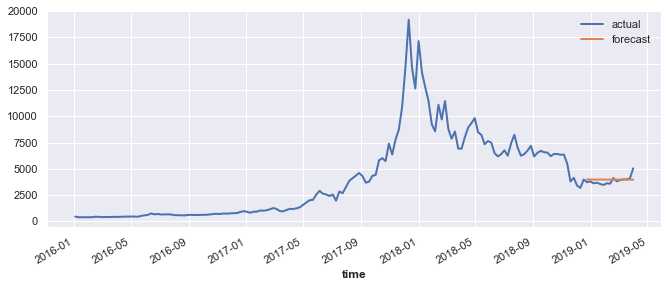
\includegraphics[width=0.45\textwidth]{Block.png}} 
    \subfigure{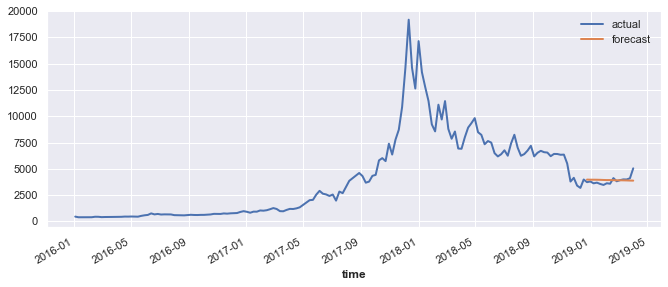
\includegraphics[width=0.45\textwidth]{transformer.png}} 
    \caption{(a) BlockRNNM (b) TransformerModel}
    \label{fig:foobar}
\end{figure}
\section{References}
\begin{itemize}
\item [1.] VADER: A Parsimonious Rule-based Model for Sentiment Analysis of Social Media Text
(by C.J. Hutto and Eric Gilbert)
Eighth International Conference on Weblogs and Social Media (ICWSM-14). Ann Arbor, MI, June 2014. https://github.com/cjhutto/vaderSentiment
\item [2.] Darts: Darts: User-Friendly Modern Machine Learning for Time Series (by Julien Herzen and Francesco Lässig and Samuele Giuliano Piazzetta and Thomas Neuer and Léo Tafti and Guillaume Raille and Tomas Van Pottelbergh and Marek Pasieka and Andrzej Skrodzki and Nicolas Huguenin and Maxime Dumonal and Jan Kościsz and Dennis Bader and Frédérick Gusset and Mounir Benheddi and Camila Williamson and Michal Kosinski and Matej Petrik and Gaël Grosch), 2021. 
https://github.com/unit8co/darts
\end{itemize}
\appendix

\end{document}
